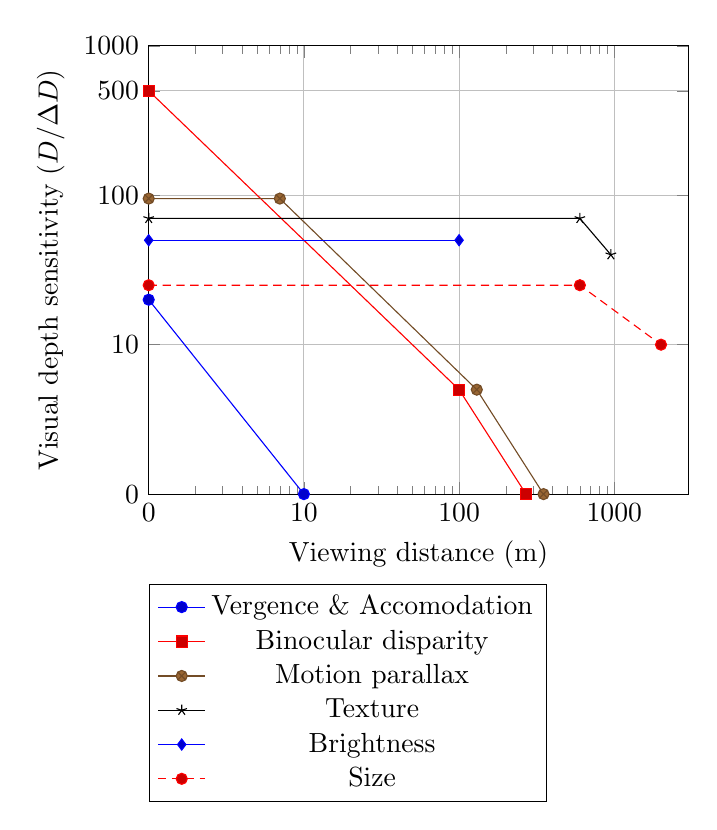
\begin{tikzpicture}
\begin{axis}[
    xmode=log,
    ymode=log,
    xmin=1, xmax=3000,
    ymin=1, ymax=1000,
    xlabel={Viewing distance (m)},
    xtick={1, 10, 100, 1000},
    xticklabels={0, 10, 100, 1000},
    ylabel={Visual depth sensitivity ($D/\Delta D$)},
    ytick={1, 10, 100, 500, 1000},
    yticklabels={0, 10, 100, 500, 1000},
    grid=major,
    legend style={at={(0.0, -0.2)}, anchor=north west}
]
\addplot coordinates {
    (1, 20)
    (10, 1)
};
\addlegendentry{Vergence \& Accomodation}

\addplot coordinates {
    (1, 500)
    (100, 5)
    (270, 1)
};
\addlegendentry{Binocular disparity}

\addplot coordinates {
    (1, 95)
    (7, 95)
    (130, 5)
    (350, 1)
};
\addlegendentry{Motion parallax}

\addplot coordinates {
    (1, 70)
    (600, 70)
    (950, 40)
};
\addlegendentry{Texture}

\addplot coordinates {
    (1, 50)
    (100, 50)
};
\addlegendentry{Brightness}

\addplot coordinates {
    (1, 25)
    (600, 25)
    (2000, 10)
};
\addlegendentry{Size}

\end{axis}
\end{tikzpicture}